\newpage
\section{Aufsetzen des Dashboards}
Zur Visualisierung der Daten wird die in Abschnitt \ref{sec:Grafana} beschriebene Open-Source-Platform Grafana genutz. Um das Grafana Dashboard mit den Daten der Hardware-Health-Monitoring Lösung zu versorgen wird das \textit{SimpleJson} Plugin verwendet. Dieses liefert eine Datenquelle, welche \ac{http} Anfragen an eine REST \ac{api} Stellt. Die Antworten dieser Anfragen werden dann als \ac{json} Dashboard bereitstehen.\\
Um die Datenquelle in Grafan nutzen zu können, muss diese zunächst konfiguriert werden. Dies kann Unter dem Reiter \textit{Data source} in der Menüleiste der Anwendung vorgenommen werden. Abbildung \ref{fig:SimpleJSONKonfig} zeigt das Konfigurationsmenü der Datenquelle. 
\begin{center}
    \begin{figure}[h!]
        \centering
        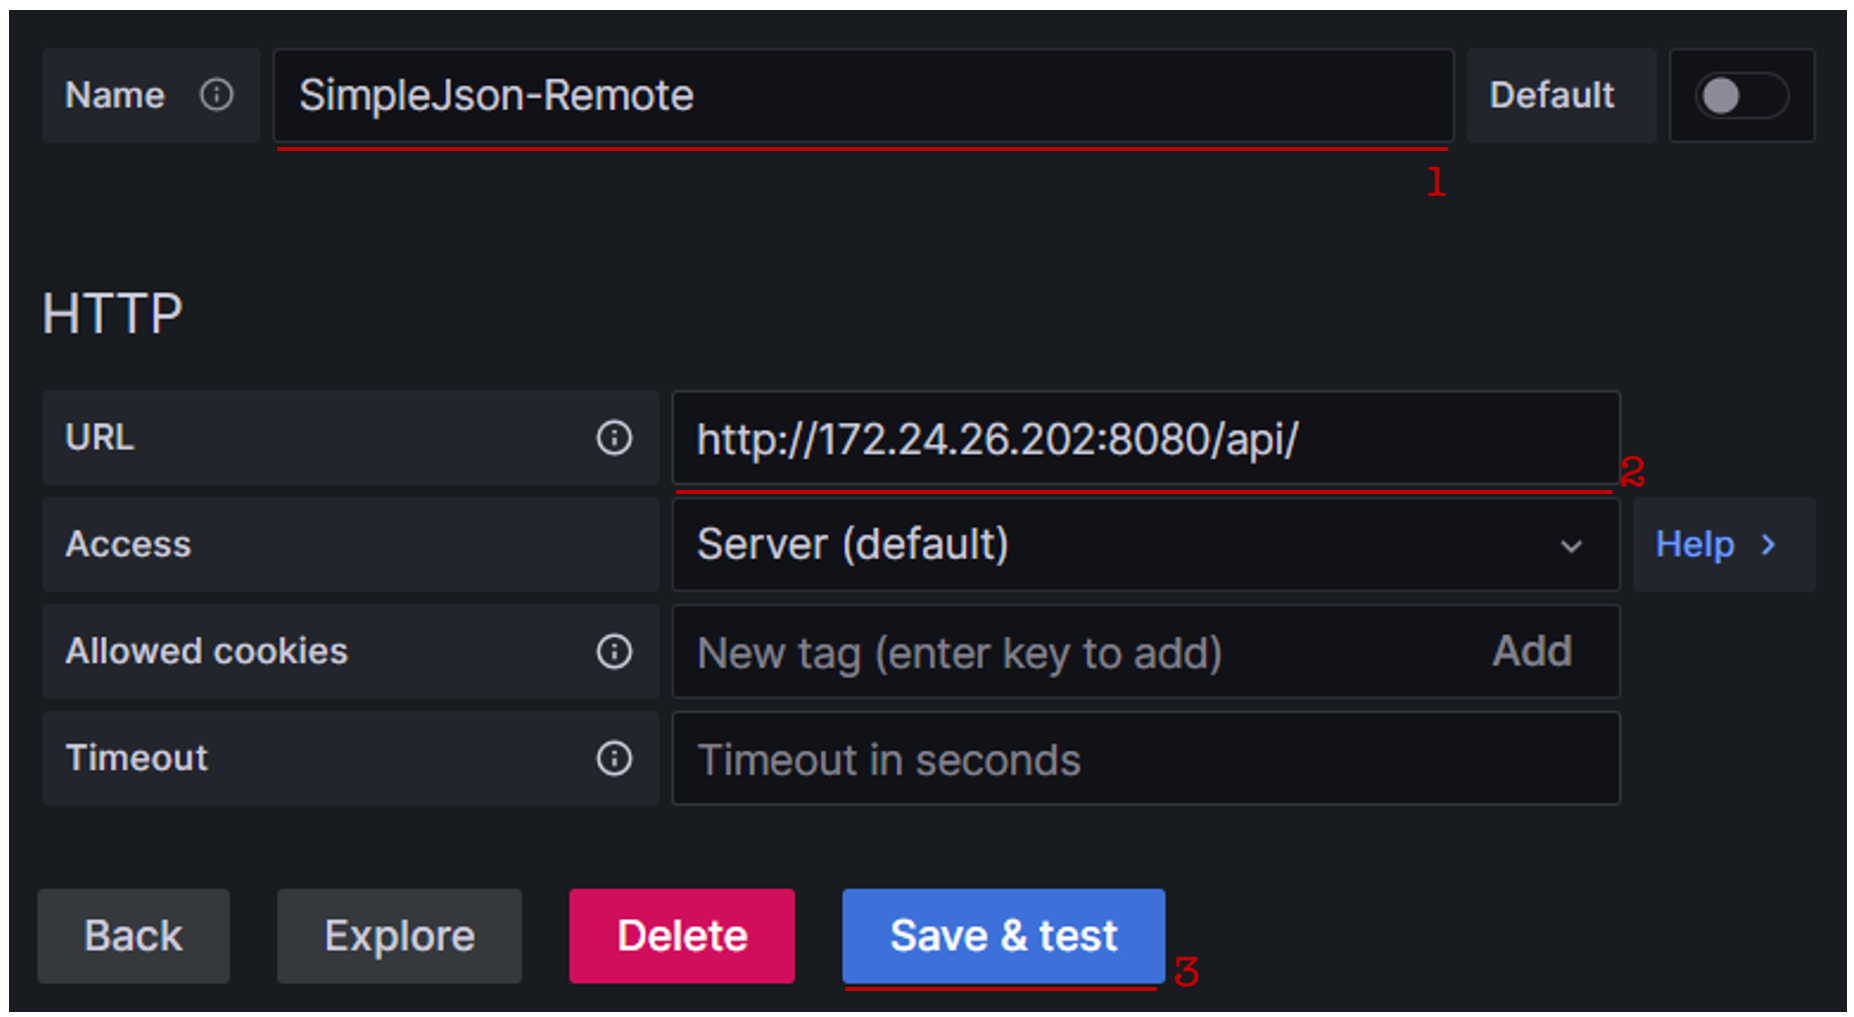
\includegraphics[width=1\textwidth]{GrafanaDatenquelle.png}
        \caption{Konfiguration der \textit{SimpleJson} Datenquelle}
        \label{fig:SimpleJSONKonfig}
    \end{figure}
\end{center}
Unter dem Feld \textit{1} im Bild \ref{fig:SimpleJSONKonfig} kann der Datenquelle ein Name vegeben werden. Anschließend wird im Feld \textit{2} die Basis URL der \ac{api} eingetragen werden. Bild zeigt nur einen abschnitt von möglichen Konfigurationsfeldern. Da dies nur ein Prototypischer Aufbau wird können die anderen Parameter offen gelassen werden. Unter den Button \textit{3} kann die Datenquelle gespeichert werden. Hierbei wird zudem direkt die Verbindung zur \ac{api} getestet.\\
Über den Menüpunkt \textit{Dashboard} kann Anschließend ein neues Dashboard erstellt werden. In diesem werden die einzelnen Panels zur visualisierung konkreter Daten erzeugt und konfiguriert. Zur visualisierung von verschiedenen Daten steht eine Reihe von Diagrammen zur verfügung.\\
Abbildung \ref{fig:PanelBearbeitung} zeigt die Ansicht, welche zur Konfiguration der einzelnen Diagramme verwendet wird.
\begin{center}
    \begin{figure}[h!]
        \centering
        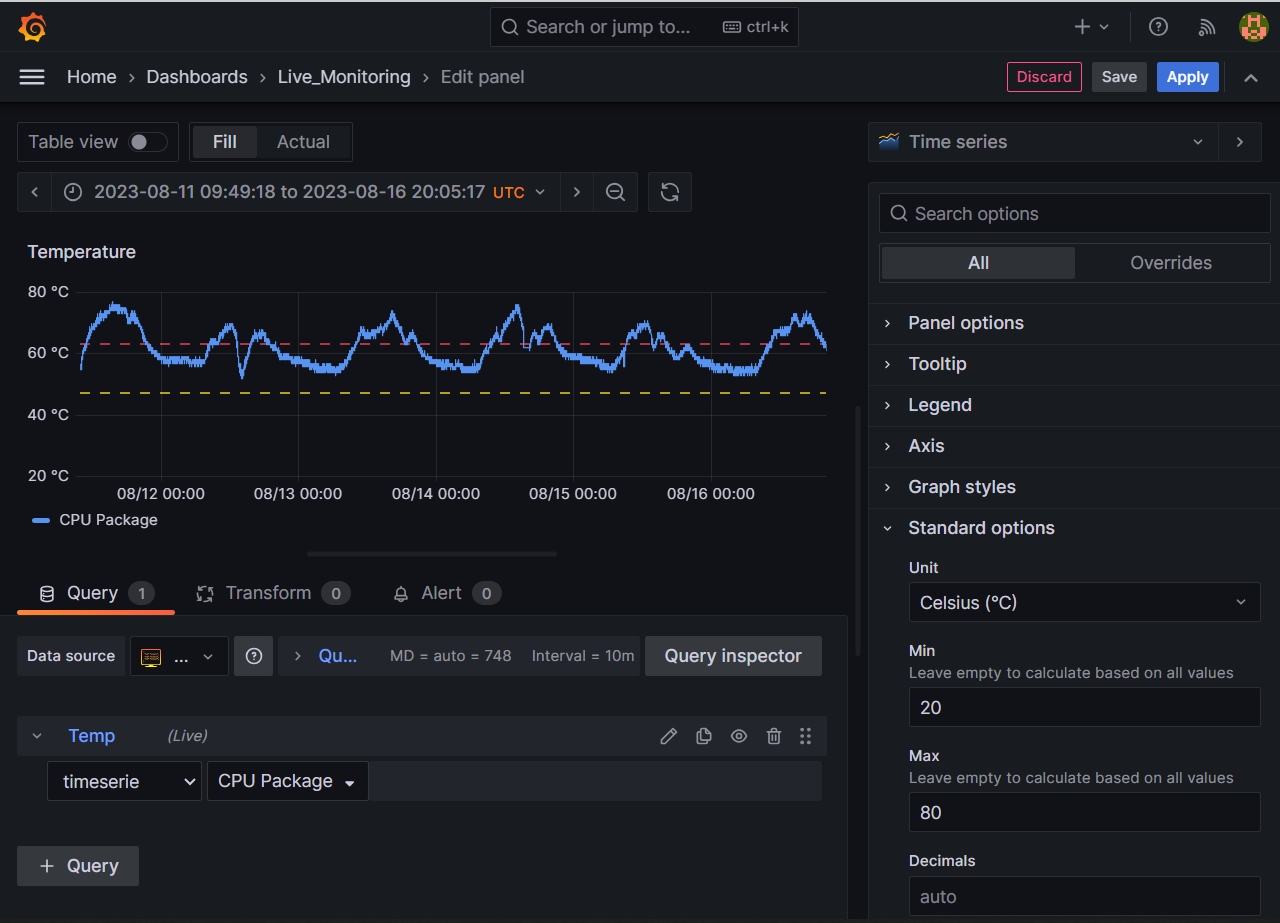
\includegraphics[width=1\textwidth]{GrafanaPanelEdit.png}
        \caption{Grafana \textit{edit panel} Ansicht}
        \label{fig:PanelBearbeitung}
    \end{figure}
\end{center}
\vspace{-1.8cm}
Zur visualisierung der einzenlen Messewerte wird das \textit{Time Series} Diagramm verwendet. Hierbei muss zunächst im Bereich links unten (Siehe Abbildung \ref{fig:PanelBearbeitung}) die zuvor erstellte Datenquelle ausgewählt werden. Anschließend wird die Anfrage Konfiguriert. Hierbei wird das Format der angefragten Daten, so wie das Label des Gewünschten Datensätze ausgewählt. Über die Rechte Spalte im bild wird Anschließend das Visuelle erscheinen des Diagrammes konfiguriert.\\
Zur visualisierung des System Status wird ein einfaches \textit{Gauge} Diagramm verwendet. Die Visualisierung der Systemstatus Historie wird mittels \textit{Pie chart} Realisiert. Die Systemzuverlässigkeit wird über ein \textit{Bar gauge} Visualisiert.\\
Abbildung \ref{fig:Grafa} zeigt das vollständige Dashboard der Anwendung.
\vspace{-2cm}
\begin{center}
    \begin{figure}[h!]
        \centering
        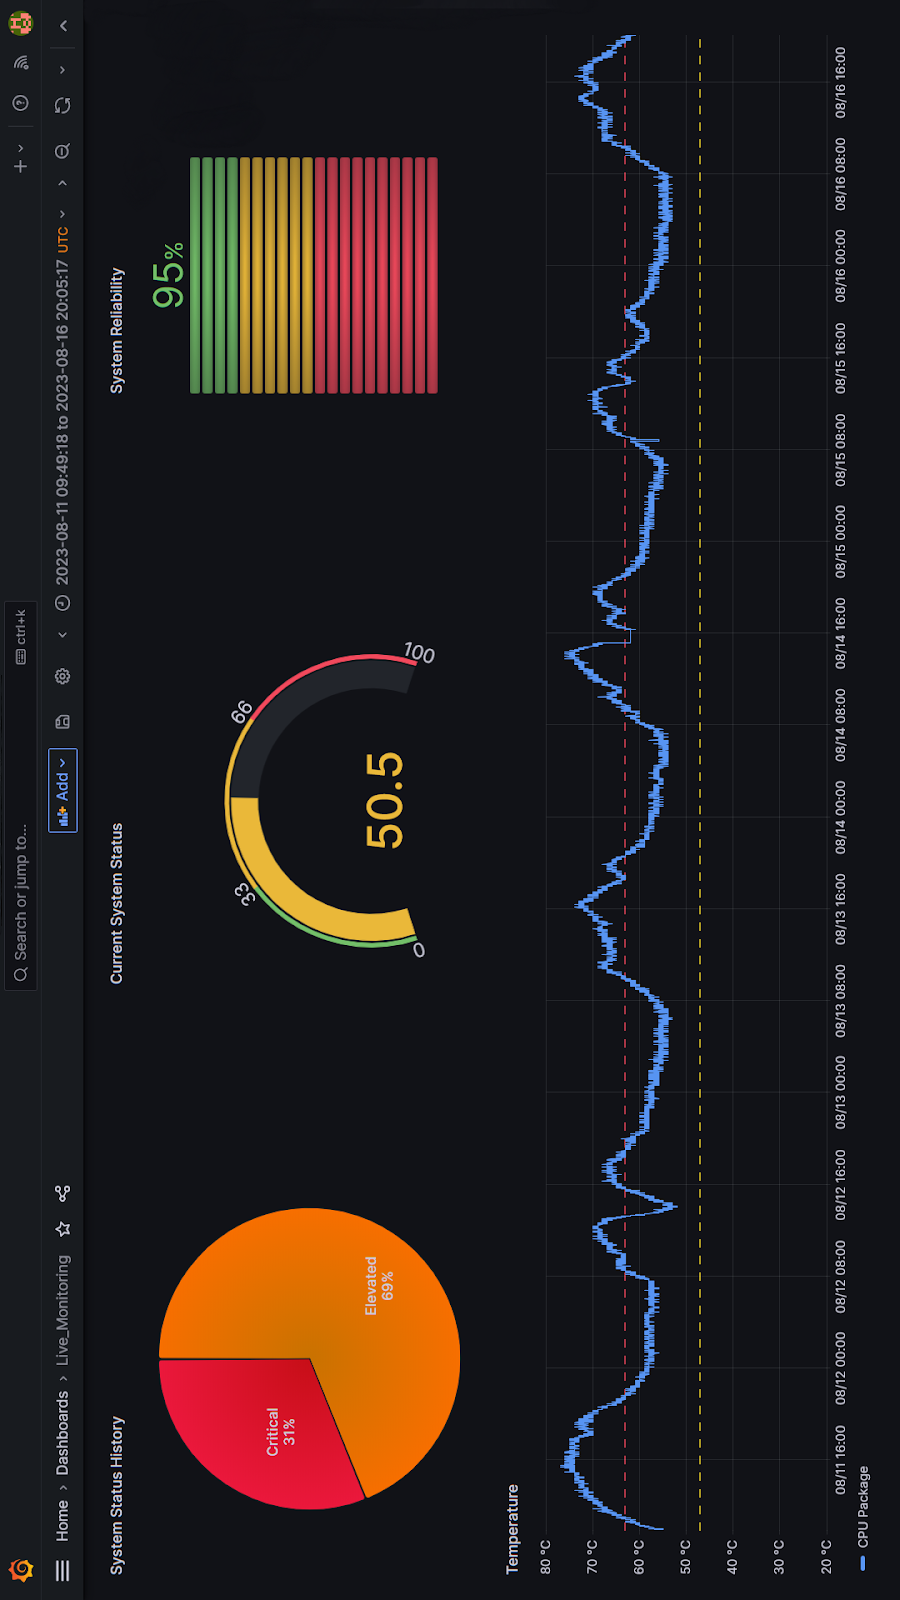
\includegraphics[height=1\textheight]{GrafanaDashboard.png}
        \caption{Grafana Dashboard der Hardware-Health-Monitoring Lösung}
        \label{fig:Grafa}
    \end{figure}
\end{center}